\documentclass[10pt,conference]{IEEEtran}
\usepackage{cite}
\usepackage{amsmath,amssymb,amsfonts}
\usepackage{booktabs}
\usepackage{array}
\usepackage{multirow}
\usepackage{tabularx}
\usepackage{graphicx}
\usepackage{tikz}
\usetikzlibrary{arrows.meta,positioning,fit,calc}
\usepackage{pgfplots}
\pgfplotsset{compat=1.18}
\usepackage{url}
\usepackage[hidelinks]{hyperref}
\definecolor{cmbInk}{RGB}{27,31,36}
\definecolor{cmbBlue}{RGB}{43,82,125}
\definecolor{cmbTeal}{RGB}{43,125,116}
\definecolor{cmbGold}{RGB}{158,116,49}
\definecolor{cmbRose}{RGB}{151,75,82}
\definecolor{cmbMist}{RGB}{239,245,249}
\definecolor{cmbMint}{RGB}{237,247,244}
\definecolor{cmbWarm}{RGB}{248,244,235}
\definecolor{cmbRule}{RGB}{196,202,205}
\definecolor{cmbGray}{RGB}{101,109,117}
\hypersetup{pdfauthor={Anonymous Authors},pdftitle={PyLockGlyph}}
\newtheorem{definition}{Definition}
\newtheorem{proposition}{Proposition}
\newcommand{\tool}{\textsc{PyLockGlyph}}
\newcommand{\Oblig}{\mathcal{O}}
\newcommand{\Req}{\mathcal{R}}
\newcommand{\Adm}{\mathcal{A}}
\newcommand{\supp}{\operatorname{supp}}
\newcommand{\admit}{\mathsf{A}}
\newcommand{\inv}{\mathsf{inv}}
\newcommand{\graph}{\mathsf{graph}}
\newcommand{\SubjectCount}{41}
\newcommand{\PackageCount}{2,050}
\newcommand{\InventoryEligible}{13}
\newcommand{\GraphEligible}{8}
\newcommand{\ProjectionDecisions}{820}
\newcommand{\ProjectionOver}{341}
\newcommand{\ConsumerBaselineDecisions}{1640}
\newcommand{\ConsumerBaselineOver}{682}
\newcommand{\ControlledCases}{971}
\newcommand{\ProofDecisions}{2,560}
\newcommand{\UnitTests}{121}

\begin{document}
\title{Python Lockfiles as Reviewable Evidence}
\author{Anonymous Authors}
\maketitle

\begin{abstract}
Python dependency tools often treat a parsed lockfile as local evidence for inventories, vulnerability matching, dependency graphs, and replay. The harder question is not whether parsing succeeds, but which downstream claims the inspected bytes actually license. A manifest/lockfile pair can name packages while omitting sources, covering only part of the integrity surface, hiding resolver-era metadata, erasing dependency edges, or drifting from the inspected manifest. \tool{} answers with profile-indexed admission verdicts. It extracts eight non-substitutable evidence types from five Python lockfile families and admits a pair only when the local facts satisfy the named consumer profile. On a frozen, benchmark-scoped corpus of \SubjectCount{} public pairs and \PackageCount{} normalized package records, only \InventoryEligible{} pairs support an inventory consumer and \GraphEligible{} support a dependency-graph consumer under explicit local evidence. Common projections that stop at parser success, coordinates, metadata, integrity, or manifest agreement over-admit \ProjectionOver{} of \ProjectionDecisions{} subject--profile decisions. A second extractor, an enumerated policy table, \ControlledCases{} targeted controls, and format-only rewrites check that decisions change only when required evidence is removed. The result is an offline, fail-closed admission check: each accepted pair states the profile it supports, and each refused pair names the missing local facts.
\end{abstract}

\begin{IEEEkeywords}
lockfile evidence, dependency graphs, Python packaging, local admission, supply-chain analysis, reproducibility
\end{IEEEkeywords}

\section{Introduction}
A modern Python project can have a manifest, a generated lockfile, hundreds of resolved packages, artifact hashes, multiple package indexes, environment markers, optional groups, VCS references, and local editable projects. Downstream tools often begin after this complexity has been flattened into a package/version inventory. Vulnerability scanners map coordinates to advisories; SBOM generators emit components; dependency visualizers derive edges; and build systems attempt installation. This workflow silently assumes that the manifest/lockfile pair is a trustworthy local representation of dependency state.

That assumption is stronger than parseability. A parser may successfully emit package coordinates when the lockfile relies on an implicit default index, when only some packages have hashes, when generated metadata has been removed, when dependency edges are unavailable, or when default direct manifest declarations no longer appear in the lock inventory. The downstream output can be internally well formed yet unsupported by the local files that were inspected. Vulnerability reachability work distinguishes declared dependencies from actually exploitable ones \cite{ponta2020vuln,pashchenko2022vuln4real}. Empirical work on dependency risk and technical leverage similarly shows that evidence must be interpreted in context rather than counted mechanically \cite{pashchenko2018matter,massacci2021leverage}. Lockfile-design work shows that formats encode materially different decisions and provenance \cite{gamage2025lockfiles}. The gap we address is the question existing pipelines usually leave implicit: \emph{is this pair locally admissible for this consumer?}

We introduce \tool, a profile-indexed admission method for Python manifest/lockfile evidence. It does not query advisories, install packages, resolve dependencies, or assert that a build is reproducible. Instead, it extracts eight required evidence types: package identity ($I$), version ($V$), explicit source anchor ($S$), artifact hash or pinned/local integrity fact ($H$), resolver epoch ($R$), dependency edge ($D$), manager metadata ($G$), and manifest agreement ($\Delta$). A consumer profile declares which types it needs. The inventory profile requires all but $D$; the dependency-graph profile requires all eight.

The payoff is operational. A scanner can distinguish parse success from inventory support, a reachability tool can demand serialized edges, and a maintainer receives the exact missing fact rather than a manager score. Because admission is a monotone predicate over a typed lattice, the rule also has a finite check surface: targeted removals, format-only rewrites, and a second extractor can all be judged against the same profile decision.

Our contributions are:
\begin{itemize}
\item \textbf{Consumer contracts for lockfile evidence.} We define local admission over eight non-substitutable evidence types and two downstream profiles, separating what a lockfile records from what an inventory or reachability consumer needs.
\item \textbf{A multi-format empirical diagnosis.} Across \SubjectCount{} public pairs and \PackageCount{} normalized records, we show which local facts are present, which are missing, and how parser-only or partial-evidence views over-authorize downstream claims.
\item \textbf{An offline stress harness.} Typed fact removals, abstract attacks, executable mutations, format-only rewrites, a second extractor, and complete policy-table checks exercise the admission rule without invoking package managers or network services.
\end{itemize}

\begin{figure*}[t]
\centering
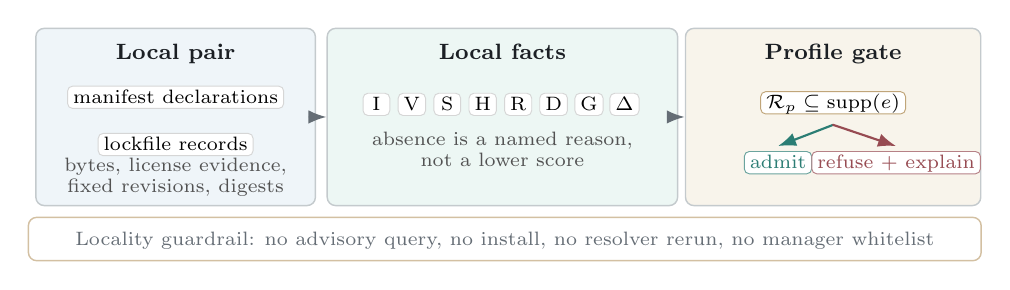
\begin{tikzpicture}[x=1cm,y=1cm,>=Latex]
\tikzset{
panel/.style={rounded corners=3pt,draw=cmbRule,line width=.52pt,inner sep=0pt},
head/.style={font=\rmfamily\bfseries\fontsize{8.0}{8.8}\selectfont,text=cmbInk,align=center,
text height=1.42ex,text depth=.30ex},
body/.style={font=\rmfamily\fontsize{6.8}{7.5}\selectfont,text=black!68,align=center,
text height=1.30ex,text depth=.28ex},
chip/.style={rounded corners=1.8pt,draw=black!16,fill=white,line width=.34pt,
font=\rmfamily\fontsize{6.6}{7.2}\selectfont,align=center,inner xsep=2pt,inner ysep=.8pt,
text height=1.24ex,text depth=.26ex},
flow/.style={->,draw=cmbGray,line width=.78pt,line cap=round,line join=round}
}
\node[panel,fill=cmbMist,minimum width=3.55cm,minimum height=2.25cm] (local) at (1.8,0) {};
\node[head] at (1.8,.82) {Local pair};
\node[chip] at (1.8,.25) {manifest declarations};
\node[chip] at (1.8,-.35) {lockfile records};
\node[body] at (1.8,-.88) {bytes, license evidence,\\fixed revisions, digests};

\node[panel,fill=cmbMint,minimum width=4.45cm,minimum height=2.25cm] (vector) at (5.95,0) {};
\node[head] at (5.95,.82) {Local facts};
\foreach \x/\lab in {4.35/I,4.80/V,5.25/S,5.70/H,6.15/R,6.60/D,7.05/G,7.50/$\Delta$}
  \node[chip,minimum width=.34cm] at (\x,.16) {\lab};
\node[body] at (5.95,-.55) {absence is a named reason,\\not a lower score};

\node[panel,fill=cmbWarm,minimum width=3.75cm,minimum height=2.25cm] (gate) at (10.15,0) {};
\node[head] at (10.15,.82) {Profile gate};
\node[chip,draw=cmbGold!65] at (10.15,.18) {$\Req_p \subseteq \supp(e)$};
\node[chip,draw=cmbTeal!70,text=cmbTeal] at (9.45,-.58) {admit};
\node[chip,draw=cmbRose!70,text=cmbRose] at (10.95,-.58) {refuse + explain};

\draw[flow] (local.east) -- (vector.west);
\draw[flow] (vector.east) -- (gate.west);
\draw[flow,draw=cmbTeal] (10.15,-.10) -- (9.45,-.37);
\draw[flow,draw=cmbRose] (10.15,-.10) -- (10.95,-.37);

\node[panel,fill=white,minimum width=12.1cm,minimum height=.55cm,draw=cmbGold!45] at (5.98,-1.55) {};
\node[body,text=cmbGray] at (5.98,-1.55) {Locality guardrail: no advisory query, no install, no resolver rerun, no manager whitelist};
\end{tikzpicture}
\caption{\tool{} turns a parsed manifest/lockfile pair into local evidence facts, then admits only the claims licensed by a named consumer profile.}
\label{fig:pipeline}
\end{figure*}

\section{Problem and Research Questions}
\subsection{The admission gap}
Package ecosystems have been studied as evolving dependency networks \cite{decan2019evolution,wittern2016dynamics,kikas2017structure}, as sources of technical lag and update pressure \cite{cox2015freshness,decan2018lag,kula2018updates}, and as operational security surfaces \cite{decan2018npmsec,zimmermann2019smallworld,vu2023badsnakes}. Open-source supply-chain attacks further show that package metadata, repository state, and update channels can become security-critical interfaces rather than neutral bookkeeping \cite{ohm2020backstabber}. Those studies assume some representation of a dependency relation or component set. Python packaging complicates that representation: PEP 440 defines version coordinates \cite{pep440}, PEP 508 defines dependency expressions \cite{pep508}, and the modern build and metadata PEPs define several interfaces that can appear without lockfile evidence for every downstream need \cite{pep517,pep518,pep621}. Emerging lock proposals make reproducible locking explicit \cite{pep665,pep751,pypaPylock}. In practice, Poetry and PDM document TOML-centered lock surfaces \cite{poetryDocs,pdmDocs}, while Pipenv, uv, and pip-tools expose different JSON, TOML, and line-oriented evidence shapes \cite{pipenvDocs,uvDocs,pipToolsDocs}.

Three failures illustrate the gap. \emph{Implicit source:} a lockfile can name and hash distributions while assuming the default Python index; an external convention is not evidence serialized by the inspected pair. \emph{Partial integrity:} hash-checking is meaningful only when integrity facts cover the relevant requirements \cite{pipHashDocs}; one hash does not cover unrelated packages. \emph{Graph erasure:} a lock can provide sources, hashes, markers, and groups while omitting transitive dependency edges. The same pair can therefore be admissible for an inventory and inadmissible for a graph consumer. These are not claims that a manager is insecure; they are mismatches between an evidence object and a consumer contract.

We ask:
\begin{description}
\item[RQ1:] Which consumer profiles are supported by the public manifest--lockfile pairs, and which local facts are absent?
\item[RQ2:] How often do parser-only or partial-evidence views authorize unsupported consumer claims?
\item[RQ3:] Do required-fact removals fail closed while format-only rewrites leave the normalized evidence unchanged?
\item[RQ4:] Does a separately written extractor produce the same inventory and evidence bits on the corpus?
\end{description}

\subsection{Boundary with downstream tools}
An admission verdict is neither an SBOM nor a vulnerability result. SPDX and CycloneDX define component-document formats \cite{spdxSpec,cyclonedxPythonDocs}; package URLs standardize component coordinates \cite{purlSpec}; pip-audit and OSV-Scanner associate packages with vulnerability records \cite{pipAuditDocs,osvScannerDocs}. SLSA frames build provenance levels \cite{slsaSpec}, while in-toto \cite{torresarias2019intoto} and TUF \cite{samuel2010tuf} protect supply-chain links and updates. NIST SSDF addresses secure-development practice \cite{nistSsdf}. Reproducible-build practice concerns deterministic correspondence after inputs have been chosen \cite{reproBuilds}. \tool{} occupies an earlier layer: it asks whether the local pair establishes the input facts required by a named analysis.

\subsection{Design requirements}
The admission layer must not replace one opaque assumption with another. We derive five requirements. \textbf{DR1--Locality:} use only the manifest, lockfile, and declared profile; no index, advisory, resolver, or build call. \textbf{DR2--Typed explanations:} rejection names missing evidence types rather than returning a scalar score or generic error. \textbf{DR3--Profile sensitivity:} adequacy is consumer-specific. \textbf{DR4--Format-neutral meaning:} adapters may extract differently, but an evidence type has one meaning. \textbf{DR5--Executable falsifiability:} removing a required type from an eligible state must reject, while irrelevant formatting must preserve the decision.

These requirements rule out tempting shortcuts. A known default registry violates locality; a weighted score permits cross-type compensation; a manager whitelist confounds format capability with evidence in one file; and an evaluation containing only naturally occurring rejections does not prove sensitivity to a particular missing type.

\subsection{Four consumer scenarios}
An advisory lookup may require names, locked versions, source identity, complete integrity, epoch metadata, and manifest agreement but not edges. Dependency reachability additionally requires edges. An SBOM producer may use the same inventory profile while attaching the admission record to its output. Build replay requires more than either profile---interpreter, platform, markers, indexes, source archives, build backends, and deterministic behavior---so \tool{} refuses to promote either studied profile into a build guarantee. The profile boundary therefore avoids both over-admission and unnecessary rejection.

\section{Local Evidence Profiles}
\subsection{Evidence Types and Profile Requirements}
Let the obligation universe be
\begin{equation}
\Oblig=\{I,V,S,H,R,D,G,\Delta\}.
\end{equation}
For a parsed pair $x$, the extractor returns a Boolean vector $e_x\in\{0,1\}^8$. Its support $\supp(e_x)\subseteq\Oblig$ contains exactly the locally present evidence types. We order vectors componentwise: $e\preceq e'$ iff $\supp(e)\subseteq\supp(e')$. Thus $\{0,1\}^8$ is a finite Boolean lattice.

A consumer profile $p$ declares a required set $\Req_p\subseteq\Oblig$. We study
\begin{equation}
\Req_{\inv}=\Oblig\setminus\{D\},\qquad \Req_{\graph}=\Oblig.
\end{equation}
The admission predicate is
\begin{equation}
\admit_p(x)=1 \Longleftrightarrow \mathrm{parsed}(x)\land\mathrm{nonempty}(x)\land \Req_p\subseteq\supp(e_x).
\label{eq:admission}
\end{equation}
The admissible region $\Adm_p=\{e\mid\Req_p\subseteq\supp(e)\}$ is the principal filter generated by $\Req_p$.

\begin{figure}[t]
\centering
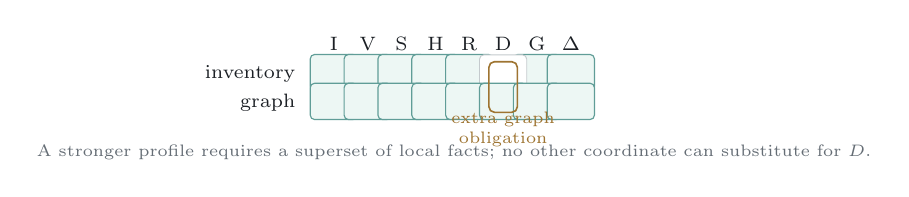
\begin{tikzpicture}[x=.43cm,y=.42cm]
\tikzset{
req/.style={rounded corners=1.6pt,draw=cmbTeal!75,fill=cmbMint,line width=.42pt,
font=\rmfamily\bfseries\fontsize{6.6}{7.2}\selectfont,align=center,minimum width=.60cm,minimum height=.38cm,
text height=1.24ex,text depth=.26ex},
gap/.style={rounded corners=1.6pt,draw=cmbRule,fill=white,line width=.34pt,
font=\rmfamily\fontsize{6.4}{7.0}\selectfont,text=cmbGray,align=center,minimum width=.60cm,minimum height=.38cm,
text height=1.20ex,text depth=.24ex},
label/.style={font=\rmfamily\fontsize{6.8}{7.5}\selectfont,text=cmbInk,anchor=east,
text height=1.30ex,text depth=.28ex}
}
\foreach \i/\lab in {1/I,2/V,3/S,4/H,5/R,6/D,7/G,8/$\Delta$}
  \node[font=\rmfamily\fontsize{6.6}{7.2}\selectfont,text=cmbInk] at (\i,2.1) {\lab};
\node[label] at (.15,1.22) {inventory};
\foreach \i in {1,2,3,4,5,7,8} \node[req] at (\i,1.22) {};
\node[gap] at (6,1.22) {};
\node[label] at (.15,.35) {graph};
\foreach \i in {1,2,3,4,5,6,7,8} \node[req] at (\i,.35) {};
\draw[draw=cmbGold,line width=.58pt,rounded corners=2pt] (5.58,.02) rectangle (6.42,1.55);
\node[font=\rmfamily\fontsize{6.4}{7.0}\selectfont,text=cmbGold,align=center] at (6,-.50) {extra graph\\obligation};
\node[font=\rmfamily\fontsize{6.5}{7.1}\selectfont,text=cmbGray,align=center] at (4.55,-1.18) {A stronger profile requires a superset of local facts; no other coordinate can substitute for $D$.};
\end{tikzpicture}
\caption{The graph profile refines the inventory profile by adding dependency-edge evidence. Each admissible region is upward closed.}
\label{fig:lattice}
\end{figure}

\subsection{Evidence meaning}
$I$ and $V$ require every normalized package record to have a canonical identity and locked version. $S$ requires an explicit package source, lock-level source list, or manifest source table; the conventional default index is not promoted into evidence. $H$ requires every package to have an artifact hash or pinned/local source fact. $R$ requires a schema, revision, generated-content hash, or equivalent resolver-era marker. $D$ requires at least one normalized package-to-package relation. $G$ requires manager-specific generated metadata rather than file-extension inference. $\Delta$ requires every default direct manifest dependency to appear in the lock inventory. Optional groups are retained diagnostically but do not silently enlarge the default installation set.

\begin{table*}[t]
\caption{Required evidence types, operational facts, and forbidden substitutions.}
\centering\small
\begin{tabularx}{\textwidth}{p{0.11\textwidth}X X}
\toprule
Type & Witness rule & Evidence that does \emph{not} substitute\\
\midrule
Identity ($I$) & Every normalized package record has a canonical nonempty name. & File name, table position, or a manifest declaration without a locked record.\\
Version ($V$) & Every package record has a locked version or commit-resolved source coordinate. & An unconstrained requirement, latest-version lookup, or parser default.\\
Source ($S$) & Explicit registry/source table, package source object, direct URL, VCS reference, or local source pointer. & An implicit default index, local machine configuration, or package name alone.\\
Integrity ($H$) & Every package has an artifact hash or pinned/local source fact. & One hash elsewhere in the file, TLS transport, or an unpinned branch reference.\\
Epoch ($R$) & Schema, revision, generated-content hash, or equivalent resolver-era marker. & Parser library version, repository commit alone, or file modification time.\\
Edges ($D$) & At least one normalized package-to-package dependency relation is serialized. & Package order, flat group membership, manifest declarations, or prose comments.\\
Metadata ($G$) & Format-specific generated lock metadata is present and parsed. & Container naming, manager label, or adapter selection.\\
Agreement ($\Delta$) & Every default direct manifest dependency appears in the lock inventory. & Optional-group coverage, package-count similarity, or a previously recorded manifest hash without the inspected manifest.\\
\bottomrule
\end{tabularx}
\label{tab:obligations}
\end{table*}

The forbidden-substitution column is part of the admission rule, not merely implementation guidance. It blocks three common category errors: replacing local evidence with configuration knowledge, replacing a relation with co-membership, and replacing universal coverage with the existence of one fact. These distinctions are what make rejection explanations stable across managers.

\subsection{Properties and profile algebra}
\begin{proposition}[Monotonicity]
If $e\preceq e'$ and $e\in\Adm_p$, then $e'\in\Adm_p$.
\end{proposition}
\emph{Proof sketch.} $\Req_p\subseteq\supp(e)\subseteq\supp(e')$.

\begin{proposition}[Profile refinement]
If $\Req_p\subseteq\Req_q$, then $\Adm_q\subseteq\Adm_p$. Hence graph eligibility implies inventory eligibility, but not conversely.
\end{proposition}

\begin{proposition}[Typed non-substitution]
For every $o\in\Req_p$, a vector whose support is $\Req_p\setminus\{o\}$ is ineligible for $p$, regardless of which non-required types are present.
\end{proposition}

\begin{proposition}[Projection separation]
Let a projection $b$ require only $P_b\subsetneq\Req_p$. There exists a vector accepted by $b$ and rejected by $\admit_p$.
\end{proposition}
The constructive example is $\supp(e)=P_b$. We instantiate it for five projections, five managers, and two profiles, yielding 50 projection-loss cases. The replay evaluates all 256 vectors for every manager/profile cell and verifies Eq.~\ref{eq:admission}, monotonicity, refinement, and single-type non-substitution. This finite check verifies correspondence between the stated predicate and the implementation; it does not claim complete parser verification. Its role is analogous to finite-model checking \cite{holzmann1997model,clarke1999model} and executable refinement arguments in verified systems \cite{leroy2009formal,klein2009sel4}.

Profiles are ordered by required evidence: $q$ is stronger than $p$ when $\Req_p\subseteq\Req_q$. Under this convention, conjunction uses requirement union, $\Req_{p\wedge q}=\Req_p\cup\Req_q$, while common capability uses requirement intersection, $\Req_{p\vee q}=\Req_p\cap\Req_q$. A toolchain can therefore combine an organizational integrity policy with a consumer graph policy without changing manager adapters. Unlike a weighted completeness score, the lattice forbids many hashes from compensating for an absent source coordinate.

\section{Implementation}
\tool{} is a Python standard-library implementation with primary and secondary parser stacks. The primary stack reads each pair, emits normalized package records and manager metadata, derives the eight-bit vector, and computes profile decisions. The secondary stack was written separately and follows different parsing and normalization paths. Differential comparison requires the ordered package name/version inventory and all eight evidence bits to agree.

The decision kernel is intentionally smaller than the adapters: it receives a typed vector, profile, and parser status. Policy therefore contains no manager or subject identifiers, and a source audit rejects corpus-shaped literals in the kernel. Each public subject carries public provenance, a fixed revision identifier, local evidence bytes, SHA-256 digests, license evidence, and an acquisition record. Generated controls copy only the evidence pair, so unrelated repository material cannot affect a transformation.

\begin{table*}[t]
\caption{Manager-specific extraction sites used by the implementation.}
\centering\small
\begin{tabularx}{\textwidth}{p{0.08\textwidth}p{0.17\textwidth}p{0.20\textwidth}p{0.18\textwidth}X}
\toprule
Manager & Manifest & Lock packages & Metadata/epoch & Source, integrity, and relation facts\\
\midrule
Poetry & Project dependency declarations & TOML package records & generated header, lock metadata, content hash & package source table; package files and hashes; dependency tables\\
PDM & Project dependency declarations & TOML package records & metadata table, strategy, groups, content hash & package source and files; dependency tables\\
Pipenv & Default package declarations & JSON default/develop objects & manager metadata, specification marker, manifest hash & source list, index fields, per-package hashes; no transitive edges in studied files\\
uv & Project dependency declarations & TOML package records & schema, revision, requires-python & package source, wheels/sdists and hashes, dependency arrays\\
pip-tools & Input requirement declarations & compiled requirement lines & generated header and command metadata & index directives, hash continuations, origin comments; no serialized transitive graph\\
\bottomrule
\end{tabularx}
\label{tab:extract}
\end{table*}

\subsection{Normalization decisions}
Cross-format normalization is where a simple package inventory can acquire unjustified meaning. We make five choices explicit. Names are normalized only for comparison; locked version strings are retained. Registry existence is never queried, although PEP 440 and PEP 508 guide coordinate handling \cite{pep440,pep508}. Sources must be serialized: URL, named registry, direct reference, VCS reference, or local source pointer. Integrity is coverage, not presence: every package needs a hash or pinned/local fact. A Pipenv group is not a dependency edge, and explanatory pip-tools comments are not promoted to an authoritative graph. Manifest agreement compares the default direct set; optional groups remain separate.

The normalized package record contains name, version, hashes, optional source anchor, dependencies, groups, marker, and pinned/local-source flags. Adapter-specific metadata remains outside the package record and contributes only to $R$ or $G$. This avoids manufacturing cross-format equivalence.

\subsection{Manager adapters and hard cases}
Adapters differ only in fact extraction. Poetry and PDM expose structured package records, source tables or objects, generated metadata, content hashes, artifact arrays, and dependency tables. Pipenv exposes sources, indexes, per-package hashes, a manifest hash, markers, and groups, but not transitive package-to-package edges. uv exposes the full studied evidence surface in the included pairs. pip-tools is line-oriented: pinned requirements, continuation hashes, index directives, and generated metadata are usable facts, while explanatory comments are not authoritative graph edges. Across managers, markers remain package metadata, optional/development groups stay outside the default agreement set unless named by a profile, and conflicting locked versions fail closed rather than being merged into a fabricated aggregate.

\subsection{Error model and policy separation}
The parser has three externally visible states: parsed with a nonempty inventory, parsed but unusable, and error. Only the first can be admitted. Malformed syntax, a missing pair member, conflicting normalized records, or an empty inventory fails closed before evidence requirements are evaluated. Missing evidence in a usable pair is not a parser error; it yields a normal rejected verdict with a typed missing set. This distinction keeps extraction defects separate from consumer-policy failure.

The policy layer contains only the eight evidence names and profile requirement sets. It cannot inspect manager family, public origin, subject identifier, package count, or storage location. Consequently, two vectors with the same parser state receive the same decision even if they came from different formats. The complete truth table tests this extensionality directly. Manager-specific logic is confined to fact extraction and diagnostic provenance.

\subsection{Decision trace and reproducibility}
Each decision records subject, profile, vector, missing types, and parser state. Public rows link bits to package records and manager metadata; transformed rows record source pair, transformation family, targeted type, and post-transformation decision. The evidence chain is
\begin{equation}
\text{bytes}\rightarrow\text{normalized fields}\rightarrow e_x\rightarrow\admit_p(x)\rightarrow\text{aggregate}.
\end{equation}
The replay checks the arrows using byte digests, differential parsing, truth-table equivalence, and paper-data generation. No network or package-manager executable is used in the core replay.

\section{Study Design}
\subsection{Benchmark construction}
The benchmark contains \SubjectCount{} complete, commit-pinned public pairs from PDM, pip-tools, Pipenv, Poetry, and uv. Inclusion required a materialized manifest and lockfile, a verified local license file, a commit identifier, parse success, a nonempty package inventory, and byte-level agreement with the acquisition record. The screening record retains 16 excluded rows and their reasons. We selected a heterogeneous, inspectable benchmark to exercise lockfile evidence across formats. The study is benchmark-scoped admission analysis: it is not a random sample of Python projects and is not used to estimate ecosystem prevalence.

Each included subject is a unit of analysis. The primary outcomes are inventory and graph eligibility; secondary outcomes are missing evidence types and projection over-admission. We report fractions and exact counts, not manager rankings. The method follows standard experimentation guidance for measurement discipline \cite{wohlin2012experimentation}. Case-study guidance informs traceability \cite{runeson2009case} and case selection \cite{shull2008guide}, while GQM-style thinking keeps research questions tied to measured outcomes \cite{basili1994gqm}. The retained screening trail makes exclusions auditable, but the study is not a literature review.

The benchmark is deliberately smaller than ecosystem metadata platforms. Libraries.io records package, version, repository, and dependency metadata at large scale \cite{katz2020librariesio}; such sources are valuable for population questions, but they cannot answer whether a reviewed manifest/lockfile pair locally serialized a source anchor, a full integrity fact, or a dependency edge. We therefore treat each retained pair as a case with inspectable bytes, license evidence, and digests rather than as a sample drawn to estimate prevalence. This follows the empirical-standard expectation that the unit of analysis and claim boundary be explicit \cite{ralph2021sigsoft}. It also follows benchmark guidance that a benchmark should define the decision it makes repeatable, not merely collect convenient examples \cite{hasselbring2021benchmarking}.

\subsection{Sampling rationale and heterogeneity}
The sample is deliberately heterogeneous along representation dimensions that exercise the construct: structured TOML, structured JSON, and line-oriented requirements; locks with and without explicit sources; artifact-hash arrays and continuation hashes; native dependency tables and flat inventories; legacy manager metadata and current schemas; local, registry, and VCS references. Diversity is evaluated at the evidence-representation level rather than by repository popularity. A large collection of near-identical pip-tools files would increase $n$ while adding little construct coverage.

Selection is nevertheless auditable. The screening log records every considered row, inclusion status, local materialization state, and exclusion reason. Exclusions are not silently deleted. Common reasons are an incomplete manifest/lock pair, missing or unverifiable license material, an excerpt rather than a repository file, an unpinned reference, or parse failure. The corpus capsule recomputes every manifest, lock, and license digest against the acquisition record. Commit pinning prevents upstream movement from changing the replay.

The benchmark is not balanced by manager and does not support manager-effect inference. Its purpose is to test a cross-format admission rule under real syntax. We therefore separate two questions that are often conflated: whether profile-indexed admission works over heterogeneous public files, and how frequent each missing type is in a target population. The first is answered here; the second requires a probability sample and is outside the present claims.

\subsection{Narrow projections}
To test whether common partial views can authorize more than the full admission rule, we define five deterministic projections: parser success; name/version inventory; manager metadata; integrity presence/coverage; and manifest-subset agreement. They are not claimed to be exact replicas of named commercial tools. They are explicit information contracts representing views routinely consumed by scanners, SBOM tools, parsers, and repository checks. Every projection is evaluated on both profiles for every subject, producing \ProjectionDecisions{} decisions. Constructive projection-loss cases separately show that each projection can accept while the full rule rejects.

\subsection{Admission-rule stress tests}
DR5 induces six suites. \emph{Evidence removals} start from eligible public pairs and remove one required typed coordinate while preserving the parsed subject and profile contract. \emph{Adversarial vectors} remove required coordinates directly in the typed domain. \emph{Executable mutations} add partial-integrity, source-relocation, empty-inventory, and parser-state families to the typed-removal cases. \emph{Metamorphic relations} combine weakening relations with package-order, hash-order, irrelevant-metadata, and optional-group preservation. \emph{Format-only rewrites} copy each manifest and lockfile through a whitespace-preserving transform and require identical inventory, evidence, and decisions. \emph{Second-extractor comparisons} recompute all public subjects using separate parsing logic.

Mutation testing turns semantic perturbations into executable checks \cite{jia2011mutation}, and generated test-suite work gives a vocabulary for oracle coverage \cite{fraser2011evosuite}. Metamorphic testing supplies the preservation relations used for format-neutral rewrites \cite{segura2016metamorphic}. The typed-removal suite additionally follows the spirit of failure-inducing input reduction \cite{zeller2002simplifying}, property-based generation \cite{claessen2000quickcheck}, and differential testing \cite{yang2011csmith}. All generated cases call the same decision kernel used for public subjects; outcomes are not prefilled.

Typed-removal transformations are designed around evidence provenance rather than byte offsets. Removing $S$ clears the source coordinate recognized by the adapter. Removing $H$ clears artifact hashes and pinned/local facts. Removing $R$ or $G$ clears the manager's generated metadata fields. Removing $D$ clears normalized dependency relations. Removing $\Delta$ introduces a default manifest declaration that is absent from the lock inventory. The resulting vector is decided by the same fail-closed admission kernel as public subjects. This path tests policy sensitivity without making replay runtime depend on large-format pretty printing.

The abstract adversarial suite complements eligible-base removals. It enumerates every required single-coordinate removal from each eligible public base and adds one compound removal per base/profile. Abstract vectors avoid a coverage artifact: a format whose public files contain no eligible base can still be tested against the admission rule. Eligible-base removals and full vector replay therefore answer different validity questions and neither is substituted for the other.

Preservation relations reverse package order, reverse hash order, add irrelevant metadata, and reorder optional groups. These transformations should not alter the normalized inventory, evidence vector, or profile decision. Weakening relations reuse the evidence removals and must move an eligible base outside the relevant principal filter.

\subsection{Analysis plan}
The analysis reads the evidence at four levels. Profile decisions and per-manager missing-type counts answer what the retained files support. Projection comparisons report over-admission, not accuracy, because no human vulnerability label is involved. Stress tests require every weakening and preservation oracle to hold. The second-extractor check requires parser agreement and zero counterexamples in the complete finite replay. All results are deterministic; timing is descriptive and not central to the claims.

\section{Results}
\subsection{Most pairs support only part of the consumer contract}
Table~\ref{tab:profiles} reports the profile outcomes. \InventoryEligible{}/\SubjectCount{} pairs satisfy the inventory profile and \GraphEligible{}/\SubjectCount{} satisfy the graph profile. These are benchmark fractions, not population estimates. The eight graph-eligible pairs are also inventory-eligible, as required by profile refinement.

\begin{table}[t]
\caption{Benchmark composition and profile outcomes. Fractions are read within each row; they are benchmark coverage facts, not manager rankings.}
\centering\small
\begin{tabular}{lrrr}
\toprule
Manager & Pairs & Inventory & Graph \\
\midrule
PDM & 5 & 1/5 & 1/5 \\
pip-tools & 15 & 0/15 & 0/15 \\
Pipenv & 5 & 5/5 & 0/5 \\
Poetry & 10 & 1/10 & 1/10 \\
uv & 6 & 6/6 & 6/6 \\
Total & 41 & 13/41 & 8/41 \\
\bottomrule
\end{tabular}

\label{tab:profiles}
\end{table}

The missing-type diagnosis (Table~\ref{tab:missing}) explains the difference. All included pairs preserve identity, version, resolver epoch, and manager metadata. Source identity is absent in 28 pairs: 4 PDM, all 15 pip-tools, and 9 Poetry. Integrity coverage is absent in 16 pairs, dominated by pip-tools (14) and two Poetry pairs. Edges are unavailable in 21 pairs: all pip-tools, all Pipenv, and one PDM pair. Four pip-tools pairs also fail default manifest agreement. uv preserves all eight types in the included benchmark; this is a statement about these files, not a universal manager guarantee.

\begin{table}[t]
\caption{Selected missing evidence types for the graph profile. Lower counts indicate fewer observed gaps for that type in the included files; bold zeros mark no observed gap.}
\centering\small
\begin{tabular}{lrrrr}
\toprule
Manager & Source & Integrity & Edges & Drift \\
\midrule
PDM & 4 & \textbf{0} & 1 & \textbf{0} \\
pip-tools & 15 & 14 & 15 & 4 \\
Pipenv & \textbf{0} & \textbf{0} & 5 & \textbf{0} \\
Poetry & 9 & 2 & \textbf{0} & \textbf{0} \\
uv & \textbf{0} & \textbf{0} & \textbf{0} & \textbf{0} \\
\bottomrule
\end{tabular}

\label{tab:missing}
\end{table}

The strict source rule is the largest driver. A conventional installer can infer a default index, but that inference is environment knowledge. A byte-based admission rule must distinguish serialized source identity from operational convention. Similarly, complete integrity means package coverage, not a lockfile containing at least one hash.

The strata illustrate different failure modes without becoming manager scores. PDM and Poetry mostly expose the needed coordinates but often omit explicit source identity; pip-tools combines usable names, versions, and metadata with missing source, incomplete integrity, absent graph edges, and four manifest-agreement failures; Pipenv satisfies inventory while consistently lacking graph evidence; uv supplies positive bases for all typed graph weakenings in the included files. At package level, the normalized table retains hash counts, source anchors, integrity status, dependency counts, groups, and markers, so a false $H$ can be localized to uncovered records rather than reported as a manager-wide failure.

\subsection{Partial projections over-authorize}
Across \ProjectionDecisions{} subject--profile--projection decisions, the projections over-admit \ProjectionOver{} times (Table~\ref{tab:projections}). Parser, name/version, and metadata views each accept all 82 subject/profile cells but only 21 cells are profile-admissible, producing 61 over-admissions each. Integrity accepts 50 cells and over-admits 29. Manifest-subset agreement accepts 74 and over-admits 53. These overlaps are intentionally counted per projection: they describe how often each partial contract loses a required type.

\begin{table}[t]
\caption{Projection decisions and full-rule over-admission. The directional comparison is the final column, where lower is stronger and bold zero means no over-admitted subject/profile cells.}
\centering\small
\begin{tabular}{lrr}
\toprule
Projection & Accepts & Over-admits \\
\midrule
Parser & 82/82 & 61 \\
Name/version & 82/82 & 61 \\
Metadata & 82/82 & 61 \\
Integrity & 50/82 & 29 \\
Manifest subset & 74/82 & 53 \\
Source+identity & 26/82 & 5 \\
Resolver metadata & 82/82 & 61 \\
SBOM proxy & 26/82 & 5 \\
Vuln graph proxy & 16/82 & \textbf{0} \\
Repro lock proxy & 26/82 & 5 \\
\bottomrule
\end{tabular}

\label{tab:projections}
\end{table}

\begin{figure}[t]
\centering
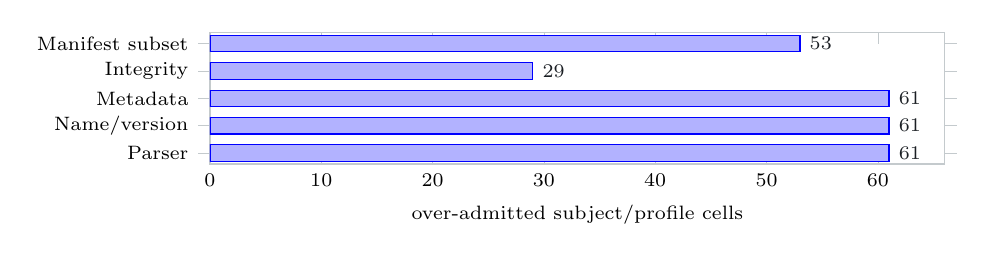
\begin{tikzpicture}
\begin{axis}[
 xbar,width=.90\columnwidth,height=3.25cm,xmin=0,xmax=66,
 symbolic y coords={Parser,Name/version,Metadata,Integrity,Manifest subset},ytick=data,
 xlabel={over-admitted subject/profile cells},xlabel style={font=\rmfamily\fontsize{6.8}{7.4}\selectfont},
 tick label style={font=\rmfamily\fontsize{6.8}{7.4}\selectfont},
 nodes near coords,nodes near coords style={font=\rmfamily\fontsize{6.7}{7.2}\selectfont,text=cmbInk},
 axis line style={draw=cmbRule},major tick style={draw=cmbRule},
 bar width=6pt,fill=cmbTeal!58,draw=cmbTeal!80]
\addplot coordinates {(61,Parser) (61,Name/version) (61,Metadata) (29,Integrity) (53,Manifest subset)};

\end{axis}
\end{tikzpicture}
\caption{Five primitive projections authorize states that lack one or more evidence types required by the named consumer. Composite consumer proxies are reported in the supplementary material.}
\label{fig:projection}
\end{figure}

The 50 projection-loss cases show that this is structural rather than accidental. For each manager, profile, and projection, the retained vector includes exactly the projection support and omits at least one profile requirement. The projection accepts and the full admission rule rejects. Public-file results then show that the theoretical separation occurs in real formats.

Projection loss can also be expressed as an information-order problem. Let $\pi_b(e)$ retain only the coordinates visible to projection $b$. If $\pi_b(e)=\pi_b(e')$ but $\admit_p(e)\ne\admit_p(e')$, then no decision procedure using only $\pi_b$ can reproduce the full admission decision on both states. Every projection-loss case is paired with an admitted vector sharing the projection view, establishing such an indistinguishable pair. The empirical over-admission counts measure how often the loss matters in this benchmark; the paired construction establishes that the limitation is unavoidable for the projection contract.

Parser and name/version projections have identical public outcomes but different interpretations. Parser success is a control-flow fact, while the name/version projection is a data fact. A separate sanity check runs two pinned consumers on 15 selected subjects, yielding 30 tool/subject rows, 12 supported attempts, and 10 parseable runs. It is not a ground-truth or accuracy study: seven disagreements are concrete tools emitting output despite missing declared obligations, and one is an external parser/environment failure on an otherwise admitted row. We use it only to anchor the projection contracts to real policy differences, not to rank tools.

\subsection{Required-fact removals fail closed}
The admission rule is sensitive to every required evidence type and invariant to irrelevant syntactic movement. Table~\ref{tab:controls} reports \ControlledCases{} controlled cases, all satisfying their oracle. Removing a required fact from an eligible base makes the corresponding profile ineligible; abstract vector weakenings reject even where the public benchmark has no eligible base for that manager/profile cell; and preservation transformations keep the normalized inventory, evidence vector, and profile decision unchanged.

\begin{table}[t]
\caption{Construct-validation suites. The intended relation is pass equals cases; bold pass counts mark suites with complete oracle agreement.}
\centering\small
\begin{tabular}{lrr}
\toprule
Validation suite & Pass & Cases \\
\midrule
Evidence removals & \textbf{155} & 155 \\
Adversarial vectors & \textbf{176} & 176 \\
Metamorphic relations & \textbf{319} & 319 \\
Executable mutations & \textbf{239} & 239 \\
Formatting transformations & \textbf{41} & 41 \\
Independent-parser comparisons & \textbf{41} & 41 \\
\bottomrule
\end{tabular}

\label{tab:controls}
\end{table}

Coverage is profile-aware. Evidence removals are generated only from a base that is eligible for the target profile, so a changed decision cannot be attributed to pre-existing ineligibility. Manager/profile cells without an eligible public base remain represented by abstract vector attacks and projection-loss cases. This separation avoids inventing a typed-removal success state that does not exist in the public benchmark.

The counts follow from the profile requirements rather than from hand-picked examples. An inventory-eligible base contributes seven single-type removals; a graph-eligible base contributes eight, and also contributes inventory removals because the consumer contract is different. The 176 adversarial vectors add one compound attack per eligible base/profile. The mutation suite contains the typed removals plus partial-integrity, source-relocation, empty-inventory, and parser-state families. Metamorphic coverage combines the weakening relations with four preservation transformations for each public pair.

No case is selected because it makes the method look favorable. Case counts deterministically follow from the included bases and requirement sets. Adding a new eligible subject automatically generates its required-type attacks; adding a new evidence type enlarges the truth table and creates non-substitution checks. This property reduces benchmark overfitting because coverage follows the admission rule rather than a hand-curated list of expected failures.

\subsection{Overfitting controls}
The study has two places where overfitting would be especially tempting: selecting files that make one manager look clean and writing tests that simply replay expected public outcomes. We avoid both. File inclusion is governed by materialization, license evidence, parseability, a nonempty inventory, and digest agreement; it is not conditioned on profile eligibility. The resulting benchmark contains eligible, partially eligible, and ineligible pairs across all five manager families. The controlled cases are generated from requirement sets and local facts after corpus construction, so the number of attacks changes automatically when a new eligible base or profile requirement is added.

The oracle design also separates public observations from rule-level claims. Public subjects show that admission decisions can be computed from real files; abstract vectors show that the set-inclusion predicate rejects every required-coordinate weakening even when a manager stratum has no eligible public base; projection-loss cases show that common partial contracts lose information before any corpus frequency is considered. These three views make the same claim falsifiable at different levels. A future corpus may change benchmark fractions, but it should not make parser success, name/version inventory, or metadata-only evidence sufficient for a graph consumer without adding the missing local facts.

\subsection{The second extractor matches corpus decisions}
The separately written parser agrees on the full ordered name/version inventory and all eight evidence bits for every public subject. The corpus comprises \PackageCount{} normalized package records. The complete finite replay evaluates \ProofDecisions{} manager/profile/vector decisions and finds zero failures for predicate equivalence, monotonicity, profile refinement, and typed non-substitution. All 50 projection-loss cases pass. The unit and integration suite executes \UnitTests{} tests, including one primary and one differential test for every public subject.

Agreement between two implementations is not proof of complete format conformance. It reduces the risk that one parser path or normalization branch determines the result, while evidence removals and truth-table replay target different failure modes. The public bytes and acquisition digests remain the ground truth for reproducibility.

The timing experiment performs three complete passes over the 41 unmodified pairs after a cold primary parse. On the evaluation host it executes 123 subject parses in the recorded timing window; the median subject latency is a few milliseconds and the tail is dominated by larger lockfiles. Timing is not used to support a semantic claim, but it shows that admission can run as a repository preflight rather than requiring package installation. The complete research replay additionally materializes all controls, evidence tables, tests, and both documents offline.

\section{Discussion and Validity}
\subsection{Evidence lineage and failure localization}
An admission verdict is useful only if a negative decision can be traced to bytes. Every public row has four linked layers. The corpus capsule identifies public origin, fixed revision, local evidence objects, license evidence, and SHA-256 digests. The parser layer emits normalized package and metadata records. The evidence layer records eight Booleans plus manager-specific provenance. The decision layer records profile, admissibility, and an ordered missing-type list. Aggregate tables are generated from those decisions rather than copied into the paper.

This lineage distinguishes three failure loci. A \emph{materialization failure} means the pair or license evidence is absent or does not match its recorded digest; such a row cannot enter the study. An \emph{extraction failure} means the local bytes cannot produce a usable normalized object; the decision fails closed with parser state. An \emph{admission failure} means extraction succeeded but the named profile lacks one or more required local facts. Only the third is counted as an inadmissible public outcome. Collapsing these loci would make missing files, parser defects, and incomplete evidence indistinguishable.

The replay preserves excluded rows rather than deleting them, making selection pressure inspectable. It also separates acquisition from analysis. An outside evaluator can reproduce every result without network access because the included bytes, license evidence, and acquisition records are local. Public-web discovery can be repeated separately, but upstream changes do not alter the analyzed objects. This design follows the same evidence discipline as the admission rule itself: external state may produce a new corpus record, but it cannot silently modify an existing one.

Paper claims are linked to generated evidence summaries. Profile fractions come from profile outcomes, missing-type counts from evidence vectors, projection counts from paired projection/admission decisions, and validation counts from cases whose rows include expected and observed outcomes. The replay compares rendered counts with the evidence summary, so a changed corpus or validation count cannot leave a stale number in the document unnoticed.

\subsection{Counterfactual and sensitivity analysis}
If parser success, name/version inventory, or manager metadata were the admission rule, all included pairs would be accepted for both consumers. An integrity-only rule is stricter but still ignores source, edge, epoch, and agreement. These counterfactuals explain why admission is not simply a more elaborate parser: its contribution is the conjunction of typed requirements named by the consumer. Changing the source rule to accept a trusted default-index configuration would admit additional PDM, Poetry, and pip-tools pairs, but the decision would then depend on evidence outside the pair. Weakening $H$ to ``some hash exists'' would similarly change outcomes without justifying un-hashed package records.

The rule is deliberately smaller than several tempting alternatives. Inventory admissibility does not establish graph completeness, artifact authenticity, vulnerability status, or build reproducibility; graph admissibility says only that the studied local requirements and at least one normalized relation are present. A scalar score would require arbitrary weights and permit compensation between unrelated types. If a graph consumer needs dependency edges, seven present facts and one missing $D$ are not ``87.5\% reviewable''; they are insufficient for that consumer. Conversely, a flat inventory should not be rejected because it lacks a graph the consumer did not ask for. A learned classifier would inherit its training distribution, and a manager capability table would describe what a format can encode rather than what a particular file did encode. Principal filters keep the claim explicit and policy-independent.

This choice changes remediation. A missing source anchor may be repaired by serializing the configured index or direct origin; a missing integrity fact may require complete hash coverage or a pinned local reference; a missing graph may require retaining resolver output rather than inferring edges from group membership. These repairs are different engineering changes. A score would collapse them into one deficit, while the admission verdict keeps them separate enough for maintainers, package-manager designers, and downstream tool builders to act.



\subsection{Admission in practice}
A profile-indexed admission check changes how evidence moves through a toolchain. Without admission, an SBOM, advisory query, or reachability stage inherits parser assumptions. With admission, the pipeline exposes three states: parsing failed, parsing succeeded but the requested profile is incomplete, or the requested profile is admitted. Only the third state authorizes downstream reliance on those local facts.

The missing-type list is a repair plan rather than a manager score. Missing $S$ suggests retaining an explicit source table; missing $H$ suggests complete hash checking or a pinned source reference; missing $D$ may require a richer lock format or resolver trace; missing $\Delta$ suggests regenerating the lock from the inspected manifest. Three integration patterns follow: a preflight command before downstream analysis, an attached evidence record beside an SBOM or scan output, and a library predicate that lets an existing parser call the eight-bit admission rule. The profile name and policy digest should be part of verdict identity so parser upgrades cannot silently change the trust contract.

Admission remains upstream of enrichment. Querying an index can confirm existence, and resolving a project can reconstruct edges, but those operations create new evidence with their own provenance and time dependence. They should produce a different verdict rather than retroactively claim that the original pair contained the facts.

\tool{} is therefore best used as a boundary object between tools rather than as a replacement for any one of them. A lockfile producer can expose the local facts it serialized; a repository service can reject rows whose digest or license evidence no longer matches the recorded object; an SBOM or vulnerability tool can state which profile it consumed; and an auditor can replay the same profile decision without depending on the producer's machine. The contract is intentionally modest: it requires only that the consumer-visible claim name the local evidence it relies on.

\subsection{Implications}
\textbf{Tool builders} should name their evidence profile rather than equate parsing with readiness. An SBOM inventory can request $\Req_{\inv}$; reachability should request $\Req_{\graph}$ or a richer profile. \textbf{Package-manager designers} can make source identity, complete integrity facts, stable schema metadata, and dependency edges serializable because those fields have downstream value even when an installer can operate without them; PEP 751 \cite{pep751} and the PyPA lockfile specification \cite{pypaPylock} create an opportunity to encode such requirements consistently. \textbf{Maintainers} get a task-specific explanation: a pair adequate for an inventory can be inadequate for a graph, and a graph can still be inadequate for build provenance. \textbf{Supply-chain frameworks} protect build steps with provenance levels \cite{slsaSpec}, record link metadata \cite{torresarias2019intoto}, harden repository metadata against tampering \cite{torresarias2016omitting}, and protect update channels \cite{samuel2010tuf}; admission verdicts complement them by making one upstream local-evidence assumption inspectable.

The main non-goal is equally important. A refused verdict should not be read as a statement that a package is malicious, unmaintained, or uninstallable. It says that a local evidence contract is incomplete for a named consumer. This distinction matters for adoption. A package manager can keep an installer-friendly format while also exporting a richer evidence view; an SBOM tool can attach an inventory verdict without claiming graph reachability; and a scanner can request a graph profile only when its analysis actually uses transitive edges. The admission boundary therefore gives toolchains a vocabulary for partial trust instead of forcing all downstream tools to share the same notion of lockfile readiness.


\subsection{Threats to validity}
Threats to validity are explicit in the admission boundary rather than hidden in parser success. \textbf{Construct validity.} The eight evidence types operationalize reviewability for two consumers. Other consumers may need markers, platform constraints, editable-state semantics, signatures, or complete edge coverage. Profiles are explicit and extensible. The source rule is stricter than normal installer behavior because the question is local reviewability; agreement compares default direct dependencies and does not treat optional groups as default.

\textbf{Internal validity.} Parser defects could change bits. We mitigate this with a second parser, byte-level corpus capsules, typed evidence removals, formatting transformations, per-package output, complete vector replay, and regression tests. Two agreeing parsers can share a misunderstanding; manager documentation and retained bytes permit inspection. The policy kernel ignores manager and subject identifiers.

\textbf{External and conclusion validity.} The 41 projects are a purposive multi-format benchmark, not a random ecosystem sample. Manager strata differ in size and age; the 5--15 pairs per stratum are too small for manager-effect claims, so we report counts and benchmark fractions without population inference or manager ranking. Controlled outcomes are deterministic admission checks, not statistical estimates; timing depends on the host and is not central. The study supports claims about the stated profiles, included files, and implemented rule, not every future lock syntax.


\subsection{Reproducibility boundary}
The replay is intentionally narrower than acquisition: it uses included bytes, license evidence, and digests; rebuilds evidence and documents; hashes generated outputs; and avoids network enrichment. Excluded rows and ineligible pairs remain visible, so a reuse study can challenge normalization choices without reconstructing hidden selection decisions. The reproducibility unit is not a single count but the mapping from local bytes to evidence types, the policy digest selecting a profile, and the row-level explanation induced by set inclusion. Parser updates, consumer-policy updates, and benchmark updates therefore remain separate changes rather than one unreviewable before/after result.

This boundary is also why negative results are useful. A rejected pair is not a failed package and not an unsafe dependency set; it is a local-evidence statement under a named consumer contract. The same bytes can be adequate for an inventory consumer and inadequate for a graph consumer, and an online resolver may legitimately produce a stronger verdict by creating new provenance. Keeping those verdicts distinct prevents a toolchain from laundering external assumptions back into the inspected pair.

\section{Related Work}
\textbf{Dependency evidence and risk.} Dependency-network studies made package structure measurable \cite{kikas2017structure}, and ecosystem studies showed how those structures evolve across package managers \cite{decan2019evolution} and JavaScript packages \cite{wittern2016dynamics}. Libraries.io provides cross-ecosystem package and dependency metadata for broad studies \cite{katz2020librariesio}. Freshness and lag work then connected dependency evidence to update decisions: Cox et al. measure dependency freshness \cite{cox2015freshness}, Decan et al. study technical lag \cite{decan2018lag}, Mirhosseini and Parnin examine automated update pull requests \cite{mirhosseini2017prs}, and Kula et al. study security-advisory-driven migration \cite{kula2018updates}. Security studies show why the representation matters: npm vulnerability impact depends on dependency-network structure \cite{decan2018npmsec}, vulnerability reachability differs from mere declaration \cite{pashchenko2022vuln4real}, ecosystem threats can concentrate in small dependency worlds \cite{zimmermann2019smallworld}, and supply-chain attacks can exploit trust relationships around package production and update paths \cite{ohm2020backstabber}. Python-specific work on malicious packages \cite{vu2023badsnakes} and vulnerabilities \cite{alfadel2023pythonvuln} operates after package evidence has been chosen. \tool{} moves one step earlier by asking whether the inspected manifest/lock pair locally supports the evidence object a consumer wants to use.

\textbf{Packaging and lockfile formats.} Python packaging specifications define version identifiers \cite{pep440}, dependency expressions \cite{pep508}, build interfaces \cite{pep517,pep518}, project metadata \cite{pep621}, repository APIs \cite{pep503,pep691}, direct-origin records \cite{pep610}, source-distribution metadata \cite{pep643}, editable installs \cite{pep660}, extras \cite{pep685}, dependency groups \cite{pep735}, and lock formats \cite{pep665,pep751,pypaPylock}. Poetry \cite{poetryDocs}, PDM \cite{pdmDocs}, Pipenv \cite{pipenvDocs}, uv \cite{uvDocs}, and pip-tools \cite{pipToolsDocs} expose different evidence surfaces. Recent lockfile-design work compares such choices across package managers \cite{gamage2025lockfiles}. Our contribution is not another syntax inventory; it is an executable admission rule that says which local facts are sufficient for a named consumer.

\textbf{Downstream consumers and provenance.} SBOM formats such as SPDX \cite{spdxSpec} and CycloneDX \cite{cyclonedxPythonDocs} need component evidence, while Package URL gives components a common coordinate scheme \cite{purlSpec}. pip-audit \cite{pipAuditDocs} and OSV-Scanner \cite{osvScannerDocs} consume package evidence for vulnerability queries. SLSA defines provenance levels \cite{slsaSpec}, in-toto records supply-chain link metadata \cite{torresarias2019intoto}, and TUF protects update channels \cite{samuel2010tuf}. These systems are complementary: they can protect or consume evidence once it exists. Admission verdicts make the upstream local-evidence assumption explicit before those systems rely on it.

\textbf{Executable validation.} The admission kernel is small enough to validate as a finite predicate. This follows the spirit of finite-model checking \cite{holzmann1997model,clarke1999model} and executable refinement arguments in verified systems such as CompCert \cite{leroy2009formal} and seL4 \cite{klein2009sel4}. The test surface uses failure reduction \cite{zeller2002simplifying}, property-based testing \cite{claessen2000quickcheck}, differential testing \cite{yang2011csmith}, mutation testing \cite{jia2011mutation}, generated test suites \cite{fraser2011evosuite}, and metamorphic testing \cite{segura2016metamorphic}. Those techniques do not make the parsers formally verified; they make the stated admission rule falsifiable.

\textbf{Benchmarking and empirical standards.} Empirical standards ask authors to make units, constructs, and validity limits explicit \cite{ralph2021sigsoft}, and benchmarking work warns that a benchmark is useful only when its decision boundary is clear \cite{hasselbring2021benchmarking}. \tool{} follows that line: subjects are files, not projects in a population model; the measured construct is profile admissibility, not package quality; and the output is a bounded verdict, not a leaderboard. This positioning is why the paper reports exact counts and projection-loss cases instead of statistical significance tests or manager rankings.

\section{Conclusion}
A parseable Python lockfile is not automatically admissible evidence. \tool{} makes that precondition explicit: adapters extract eight local facts, profiles select non-substitutable requirements, and a principal-filter test yields a typed explanation. In a five-format public benchmark, source identity, complete integrity, and dependency relations---not package coordinates---are the decisive local gaps. Complete policy-table checks and \ControlledCases{} controlled cases reproduce the admission decisions offline. Admission therefore lets downstream tools state what they trust instead of inheriting authority from parser success.

The broader lesson is that dependency evidence should be treated as a typed interface, not as a by-product of installation. A lock can be excellent installer input while remaining insufficient for a graph consumer, and a flat inventory can support one analysis while refusing another. PyLockGlyph turns that distinction into a reproducible admission verdict that future formats can be judged against: which local facts do they actually serialize?

\section{Data Availability}
The anonymized package provides the retained manifest/lock capsules, evidence vectors, parser outputs, generated controls, projection results, excluded-row ledger, table inputs, and SHA-256 digests. Replay regenerates the profile decisions, missing-type counts, projection over-admissions, stress outcomes, and reported tables from fixed public revisions. Credentials, private machine state, author metadata, and unpublished discovery notes are excluded. The preserved archive is available at \url{https://doi.org/10.5281/zenodo.21085701}; a source mirror carries the same artifact surface.

\bibliographystyle{IEEEtran}
\bibliography{references}
\end{document}
